\documentclass[crop,tikz]{standalone}
\begin{document}
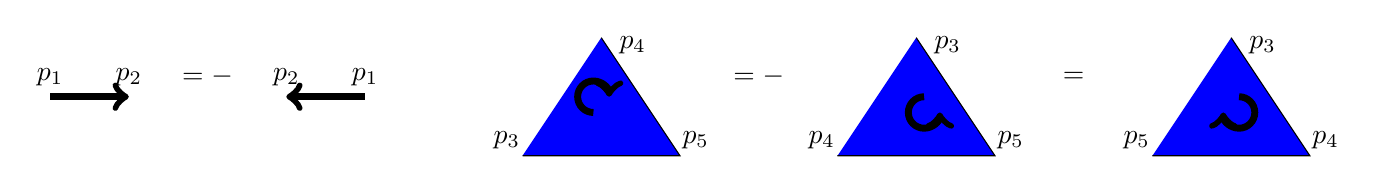
\begin{tikzpicture}
  \draw[->,line width=2.5] (1,.75) -- (2,.75);
  \draw (1,1) node{$p_1$};
  \draw (2,1) node{$p_2$};

  \draw (3,1) node{$=-$};

  \draw[<-,line width=2.5] (4,.75) -- (5,.75);
  \draw (4,1) node{$p_2$};
  \draw (5,1) node{$p_1$};


  \draw[fill=blue] (7,0) -- (9,0) -- (8,1.5);
  \draw (6.8,.2) node{$p_3$};
  \draw (9.2,.2) node{$p_5$};
  \draw (8.4,1.4) node{$p_4$};
  \draw[line width=2.5,<-] (8.1,.75) arc(0:270:.2);

  \draw (10,1) node{$=-$};

  \draw[fill=blue] (11,0) -- (13,0) -- (12,1.5);
  \draw (10.8,.2) node{$p_4$};
  \draw (13.2,.2) node{$p_5$};
  \draw (12.4,1.4) node{$p_3$};
  \draw[line width=2.5,->] (12.1,.75) arc(90:360:.2);

  \draw (14,1) node{$=$};

  \draw[fill=blue] (15,0) -- (17,0) -- (16,1.5);
  \draw (14.8,.2) node{$p_5$};
  \draw (17.2,.2) node{$p_4$};
  \draw (16.4,1.4) node{$p_3$};
  \draw[line width=2.5,->] (16.1,.75) arc(90:-180:.2);

\end{tikzpicture}
\end{document}
